
\renewcommand{\EntradaBibtex}{Ajedrez3D_2017}
%\setcounter{footnote}{0}


\begin{frame}{\citetitle{\EntradaBibtex} \footnotemark[1] (1)}
%\begin{block}{Multiplayer Chess \footnotemark} 
\begin{columns}
\begin{column}{0.4\textwidth}
		\begin{itemize}
		\item Cada pieza fue modelada en Blender y exportada a la aplicación de Android
		\item Aplicación multidispositivo, que permite llevar una partida de ajedrez.
		\item El control del juego queda del lado del servidor. 
		\end{itemize}

\end{column}
\begin{column}{0.3\textwidth}
%   some text here some text here some text here some text here some text here
     \begin{center}
     %%%%% this is a minipage, so \textwidth is already adjusted to the size of the column
     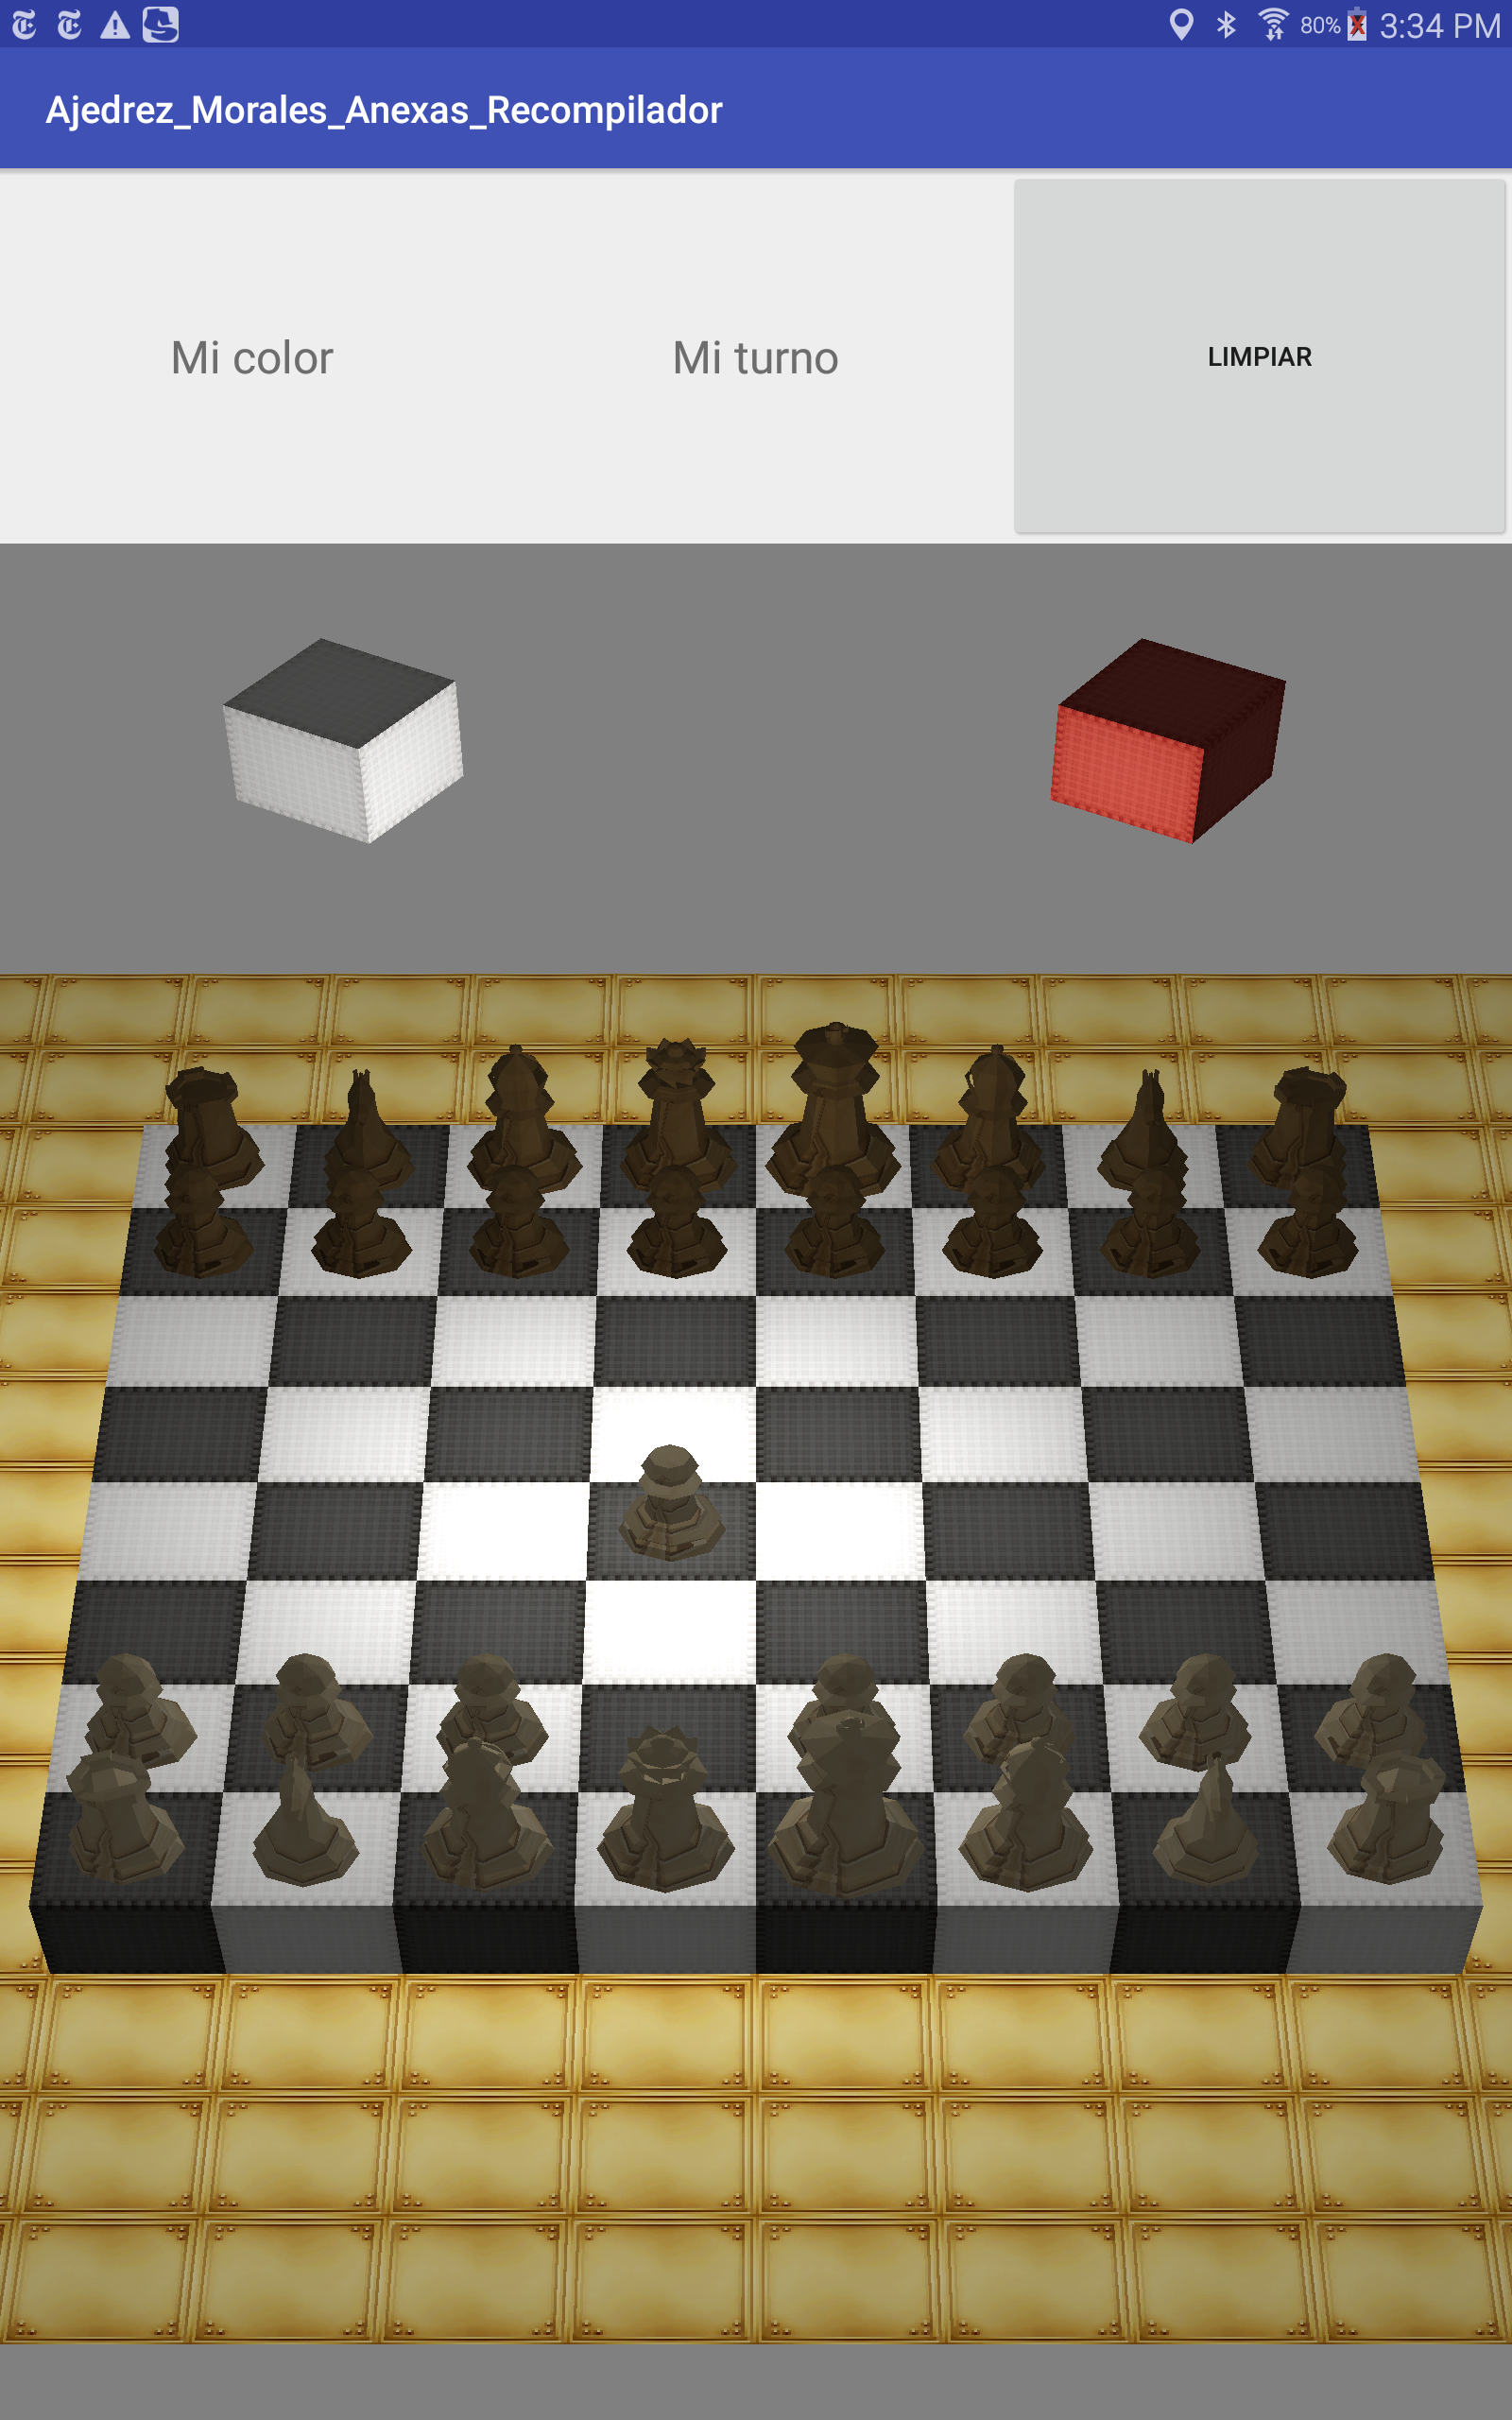
\includegraphics[width=0.7\textwidth]{Figs/Ajedrez_01}
     \end{center}

\end{column}
\begin{column}{0.3\textwidth}  
    \begin{center}
     %%%%% this is a minipage, so \textwidth is already adjusted to the size of the column
     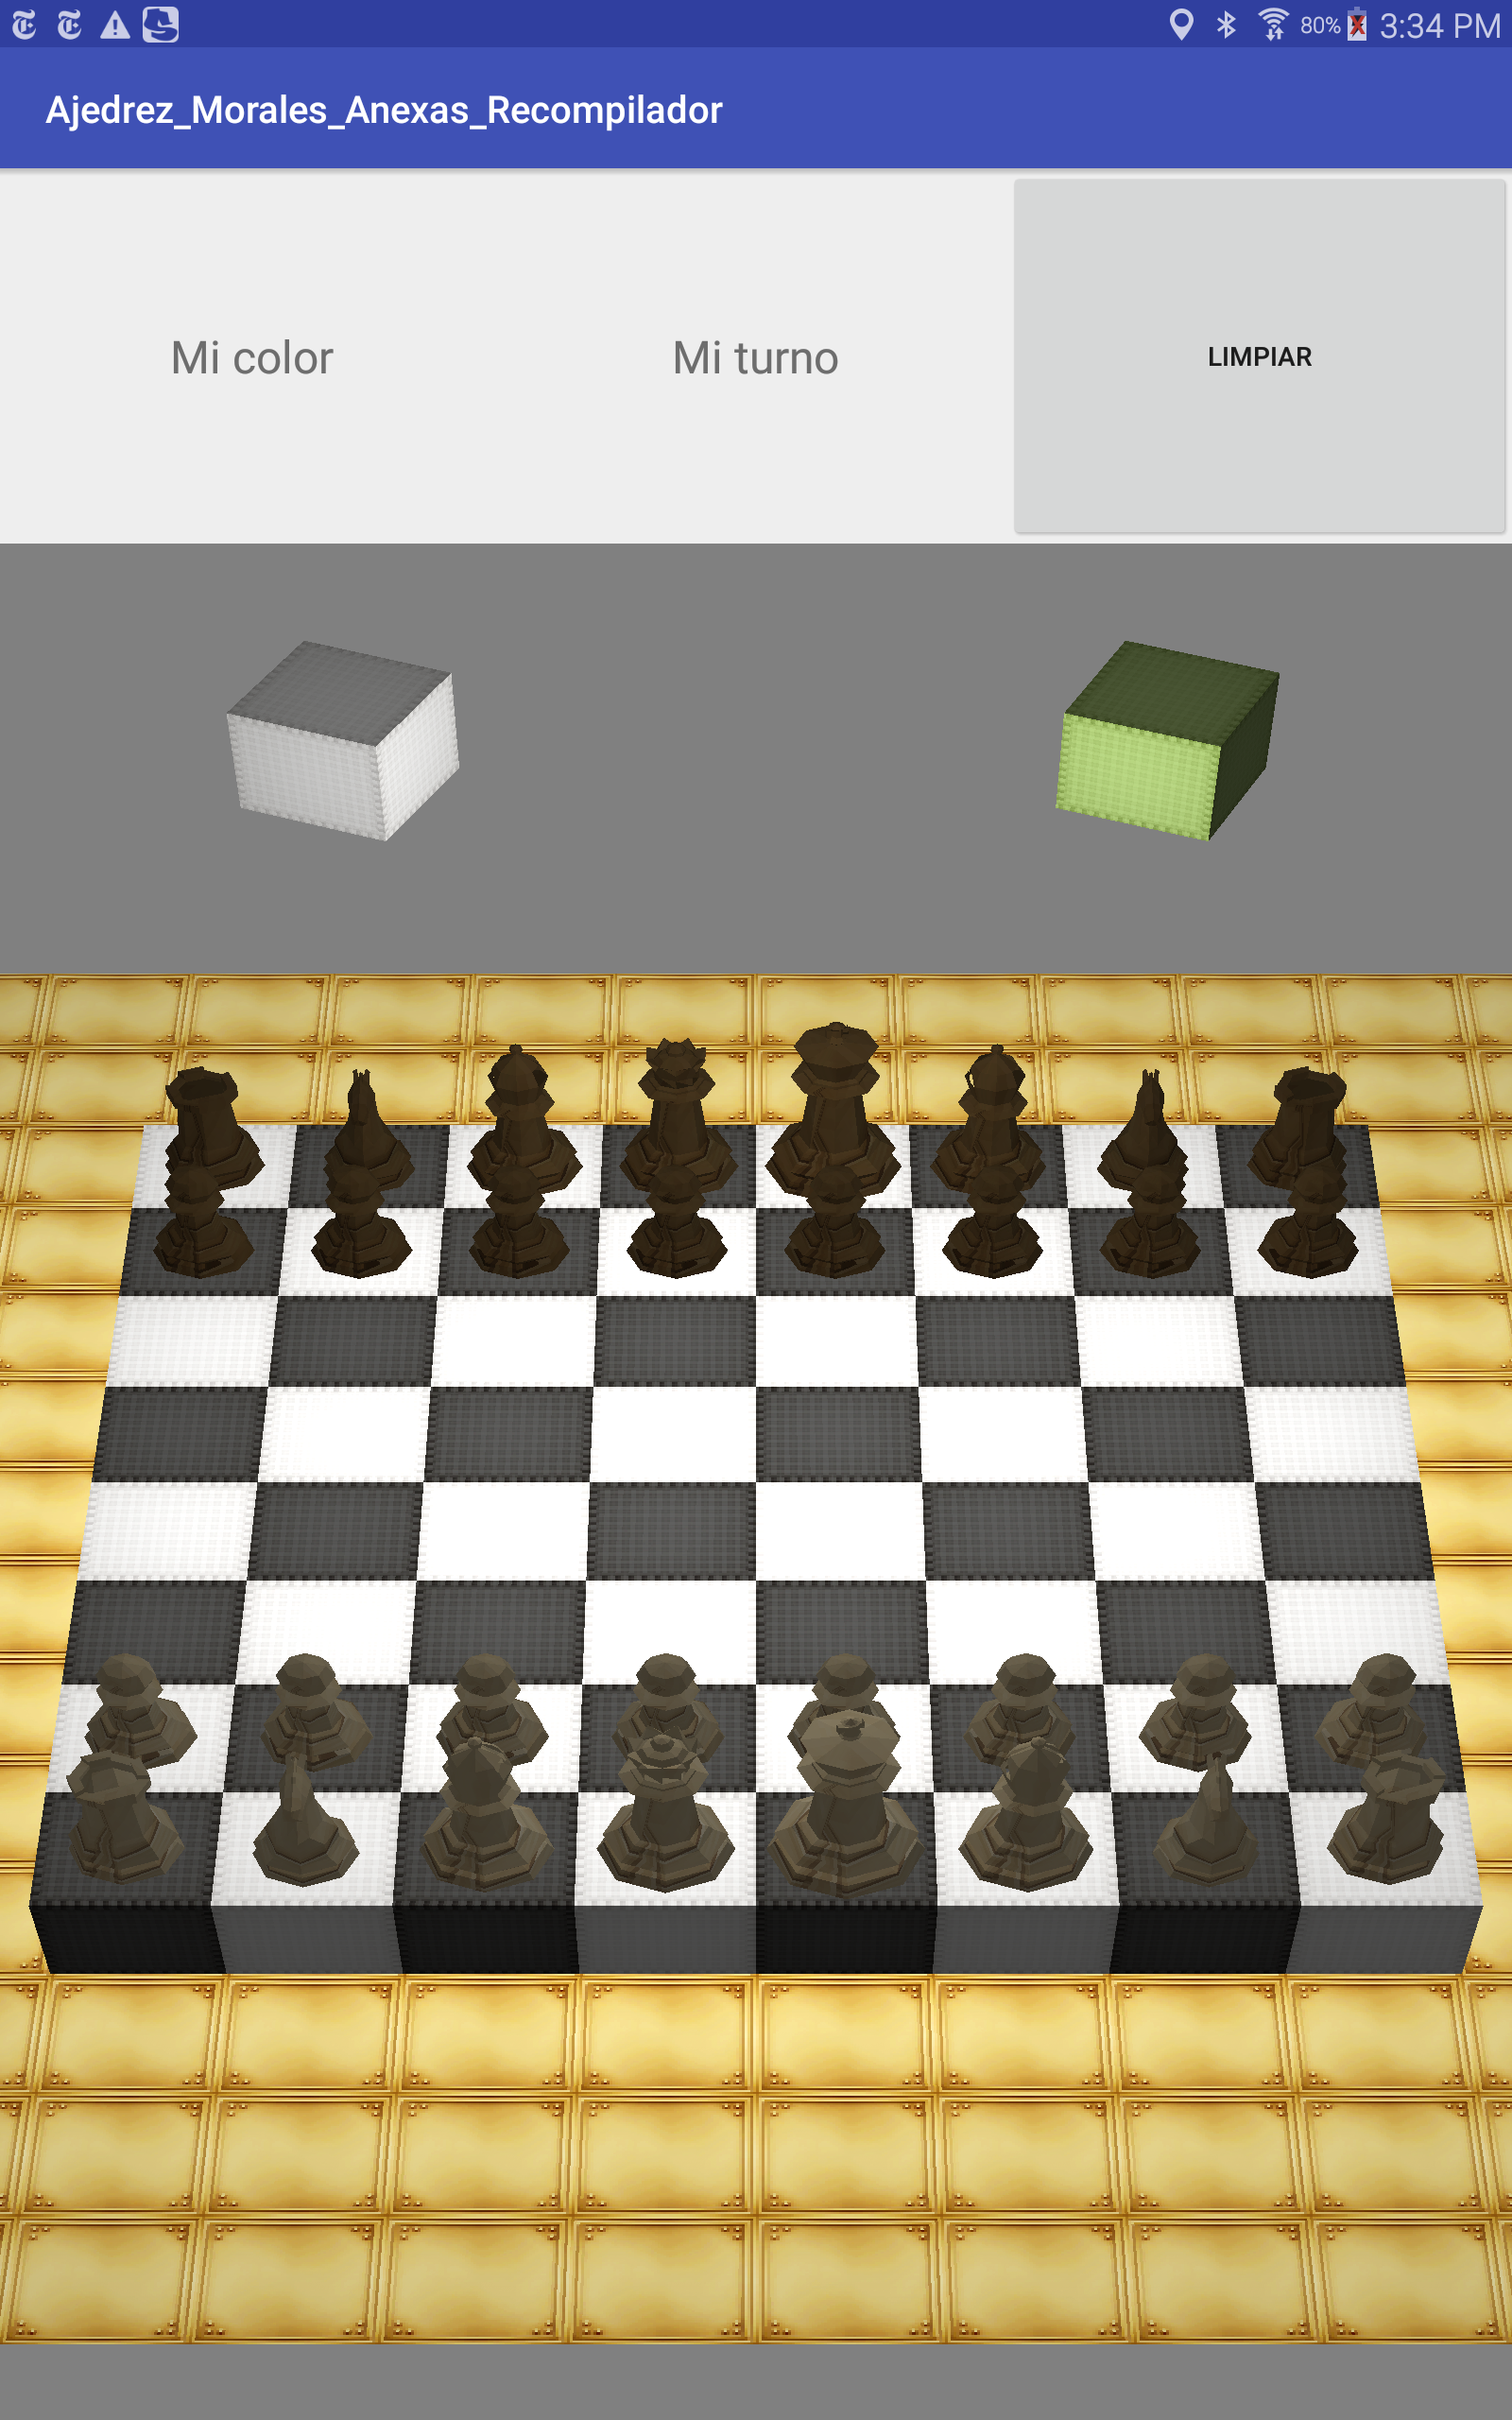
\includegraphics[width=0.7\textwidth]{Figs/Ajedrez_02}
     \end{center}
\end{column}
\end{columns}
%\footfullcite*{\EntradaBibtex}
\footnotetext[1]{\fullcite{\EntradaBibtex}}
\end{frame}

